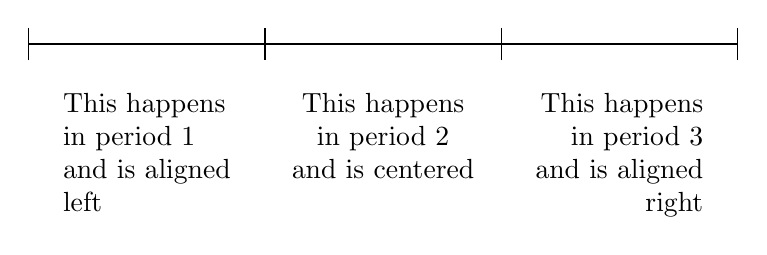
\begin{tikzpicture}
\draw [thick] (0,0) -- (9,0);
\draw (0,-0.2) -- (0,0.2);
\draw (3,-0.2) -- (3,0.2);
\draw (6,-0.2) -- (6,0.2);
\draw (9,-0.2) -- (9,0.2);
\node[align=left, below] at (1.5,-0.5) {This happens\\in period 1\\and is aligned\\left};
\node[align=center, below] at (4.5,-0.5) {This happens\\in period 2\\and is centered};
\node[align=right, below] at (7.5,-0.5) {This happens\\in period 3\\and is aligned\\right};
\end{tikzpicture}
